\documentclass{article}
\usepackage[utf8]{inputenc}
\usepackage[russian]{babel}
\usepackage[left=2cm,right=2cm,
top=2cm,bottom=2cm,bindingoffset=0cm]{geometry}
\usepackage{graphicx}
\usepackage{amsmath}
\usepackage{float}
\usepackage{listings}
\usepackage{url,textcomp}
\date{6 марта 2019 г.}
\author{Кондратенко Федор, гр 13632/1}
\setlength{\parindent}{0pt}
\setlength{\parskip}{5pt plus 2pt minus 1pt}
\frenchspacing
\title{Отчет по заданию №2.1}
\begin{document}
	\maketitle
	\section{Формулировка задания\\}
	\underline{Задачи:}
	\begin{enumerate}
		\item Написать законы движения тела в векторном виде и в проекциях на оси;
		\item Собрать в Simulink схему, моделирующую полет тела под углом к горизонту;
		\item Сделать выводы о влиянии угла броска на дальность приземления;
		\item  Определить степень влияния параметров моделирования на дальность полета.
	\end{enumerate}
	\section{Теоретическая часть}
	Закон движения в векторном виде:
	$$m\underline a = \underline G + \underline R_{sopr}$$
	В проекциях на оси:
	$$mx'' = -kx'$$
	$$my'' = -mg-ky'$$
	\section{Блок-схемы}
	В схему было введено условие остановки моделирования -- при касании поверхности (введено допущение - снаряд летит над абсолютно прямой поверхностью).
	\begin{figure}[H]
		\centering
		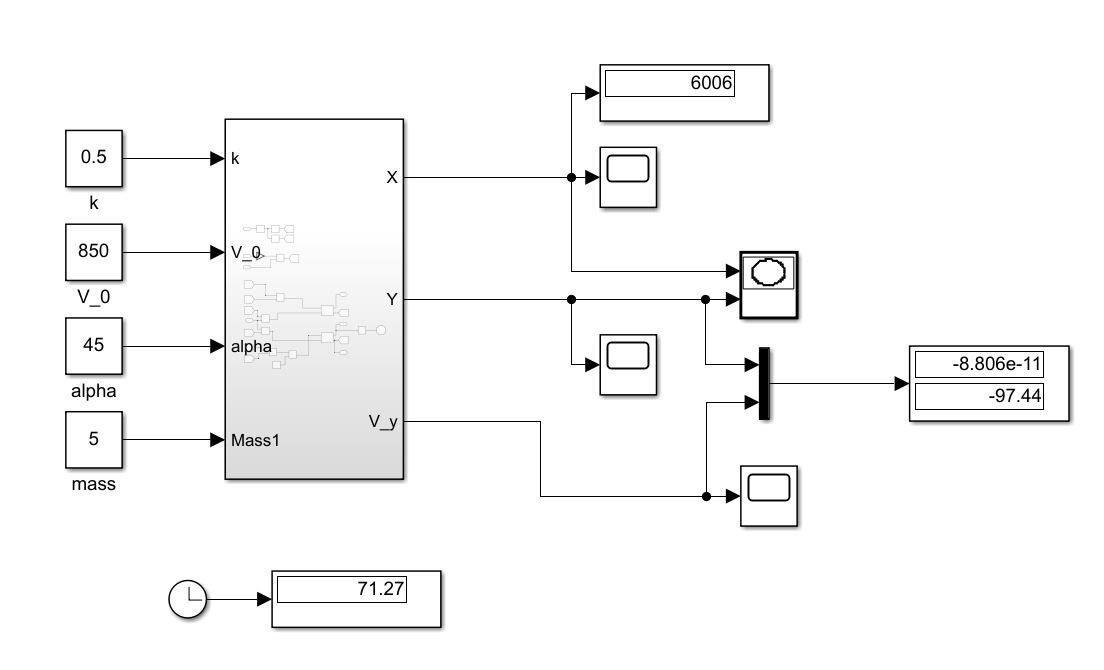
\includegraphics[width=0.7\linewidth]{model1}
		\caption{Общая схема модели}
		\label{fig:model1}
	\end{figure}
	\begin{figure}[H]
		\centering
		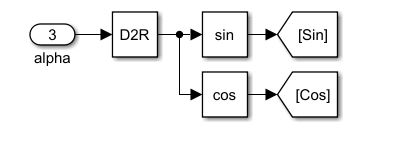
\includegraphics[width=0.7\linewidth]{model2}
		\caption{"Тригонометрическая" часть подсистемы}
		\label{fig:model2}
	\end{figure}
	\begin{figure}[H]
		\centering
		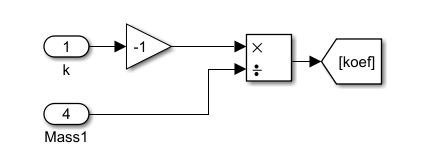
\includegraphics[width=0.7\linewidth]{model3}
		\caption{Часть подсистемы, подсчитывающая коэффициент $\frac{-k}{m}$}
		\label{fig:model3}
	\end{figure}
	\begin{figure}[H]
		\centering
		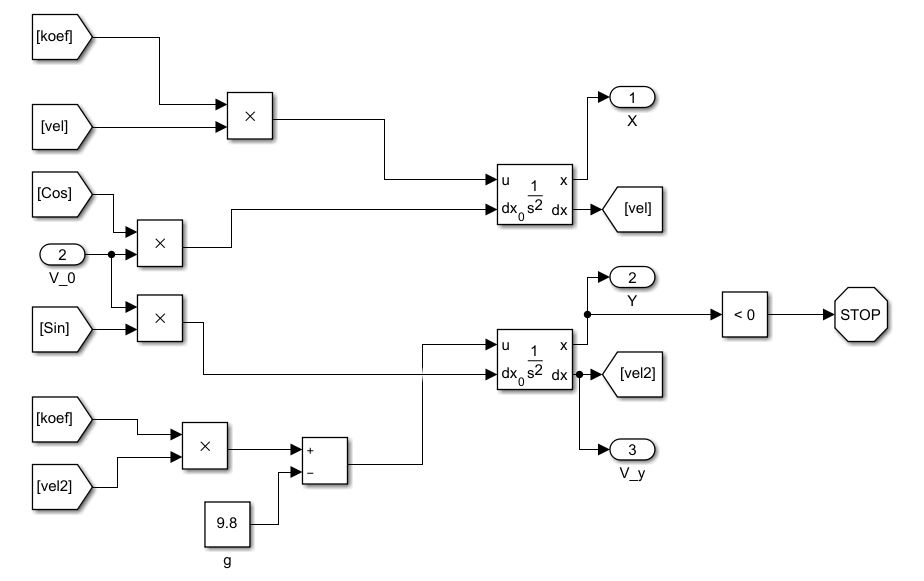
\includegraphics[width=0.7\linewidth]{model4}
		\caption{Основная часть подсистемы, где происходит интегрирование уравнений движения}
		\label{fig:model4}
	\end{figure}
	\section{Графики}
	\begin{figure}[H]
		\centering
		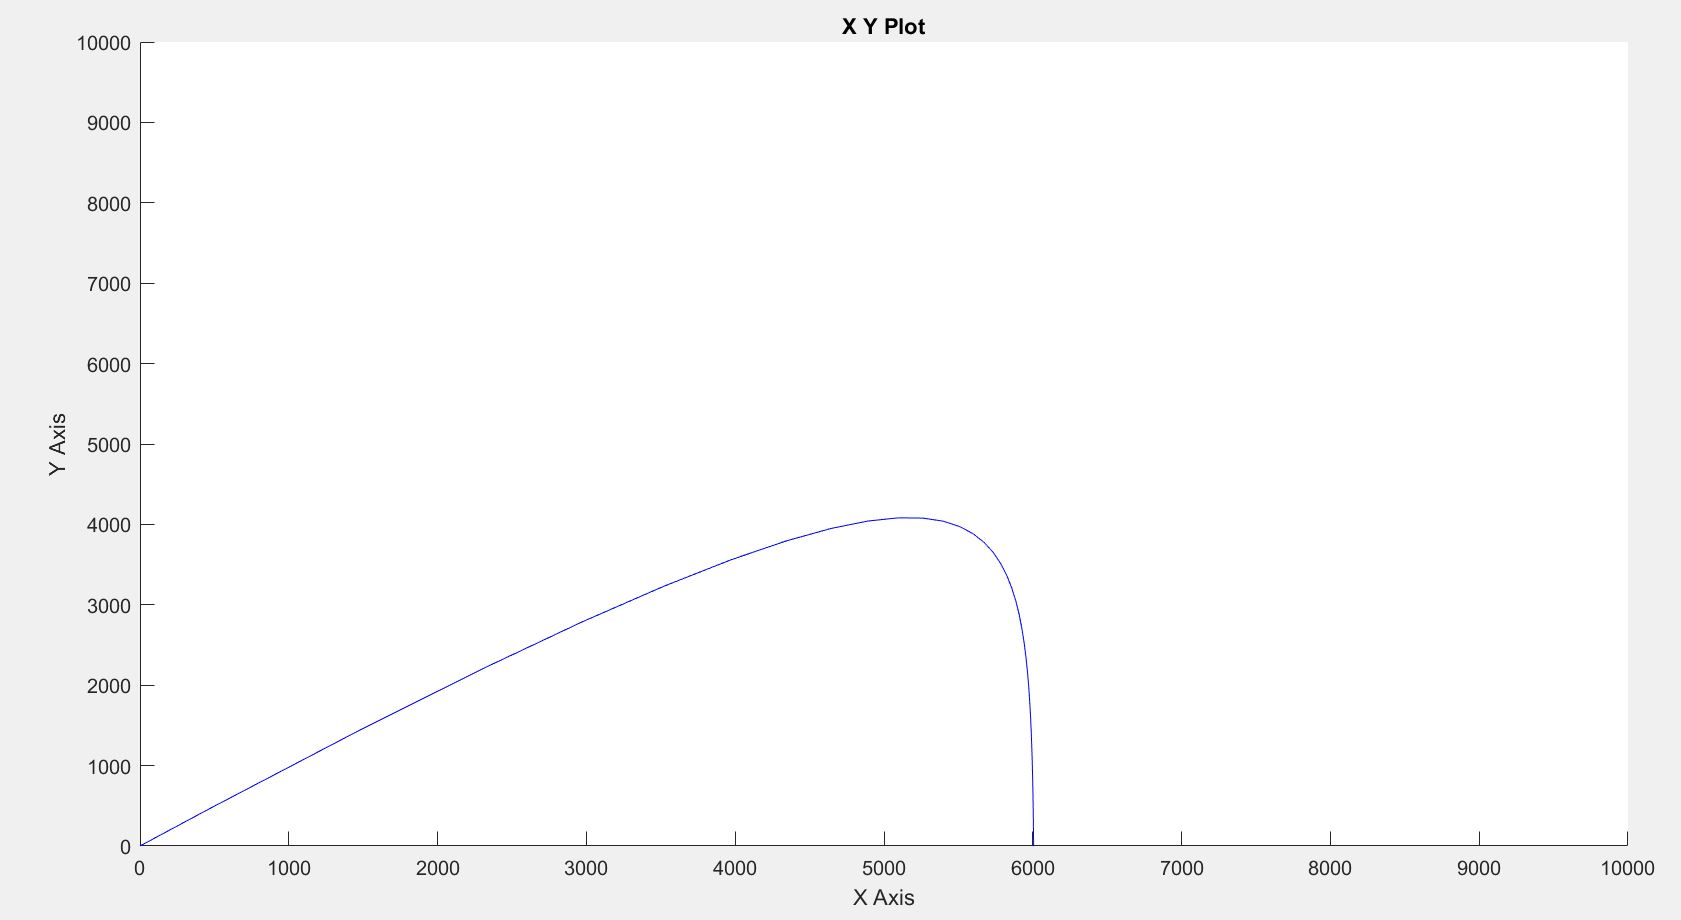
\includegraphics[width=0.7\linewidth]{graph1}
		\caption{Траектория полета снаряда с максимальной дальностью при начальных условиях $k=0.5,\ V_0 = 850\ m/s,\ m = 5\ kg,\ \alpha = 45$}
		\label{fig:graph1}
	\end{figure}
	При указанных начальных условиях дальность полета составила 6006 метров, время полета составило 71.25 секунды, максимальная высота -- 4081 метр.\\
	\begin{figure}[H]
		\centering
		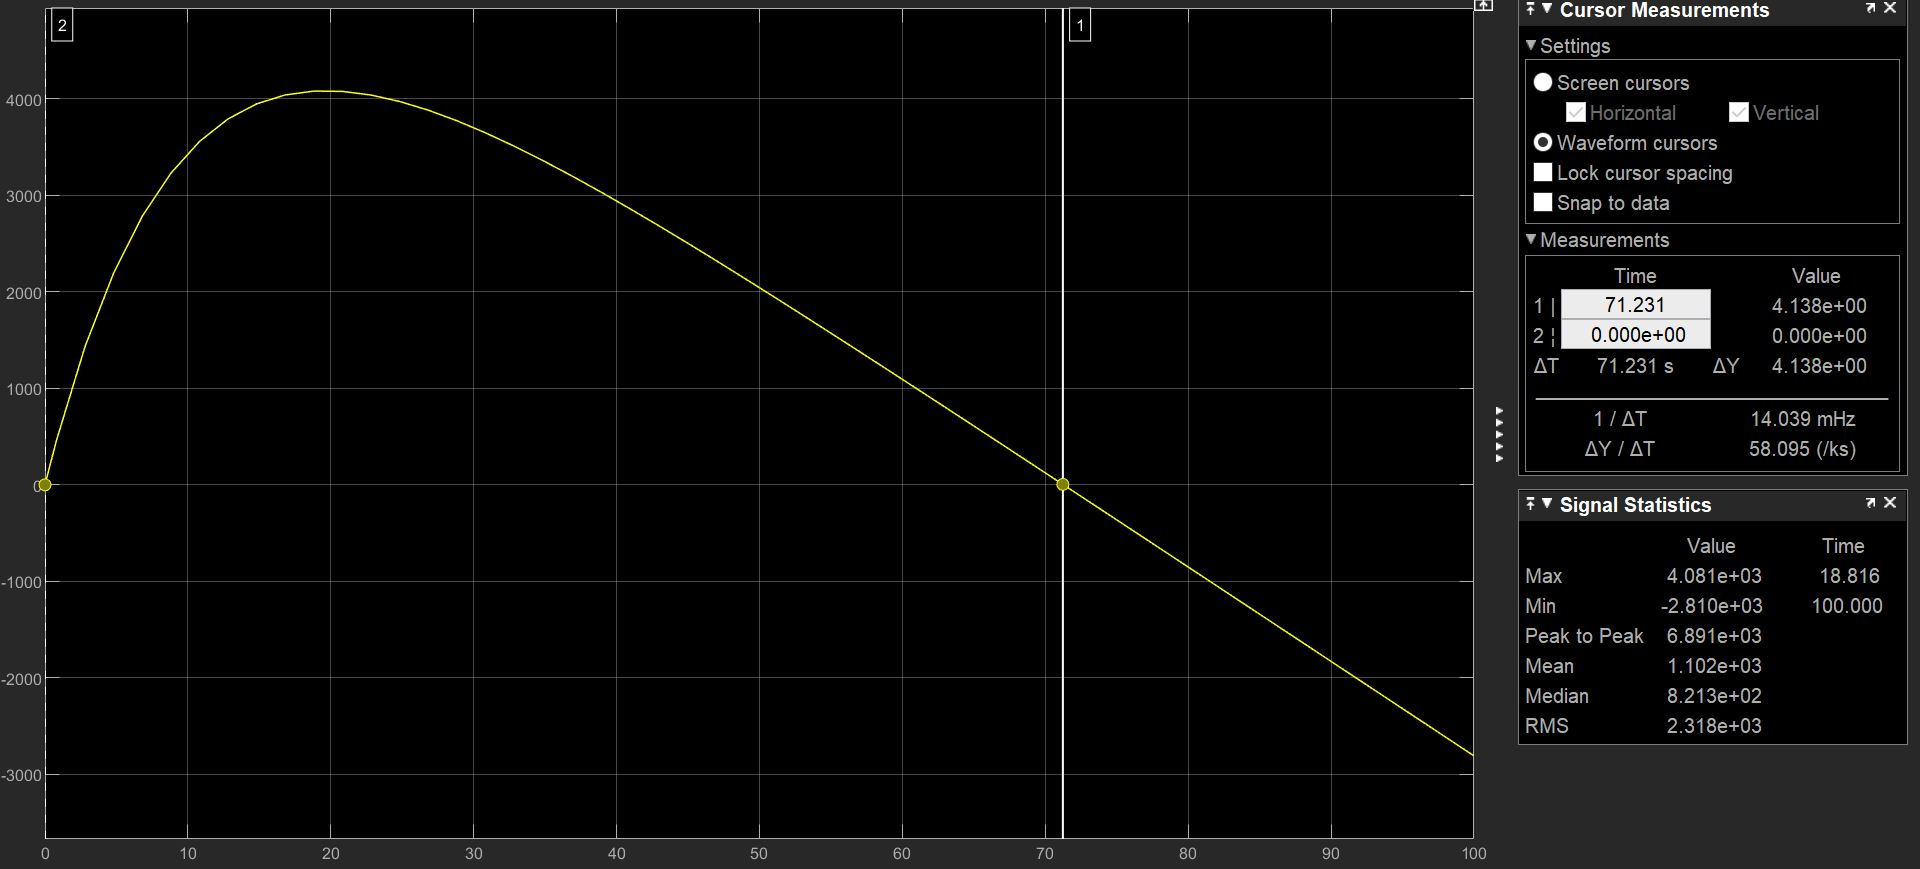
\includegraphics[width=0.7\linewidth]{data1}
		\caption{Данные анализа вертикальной составляющей траектории полета, из них получена информация о максимальной высоте.}
		\label{fig:data1}
	\end{figure}
	\begin{figure}[H]
		\centering
		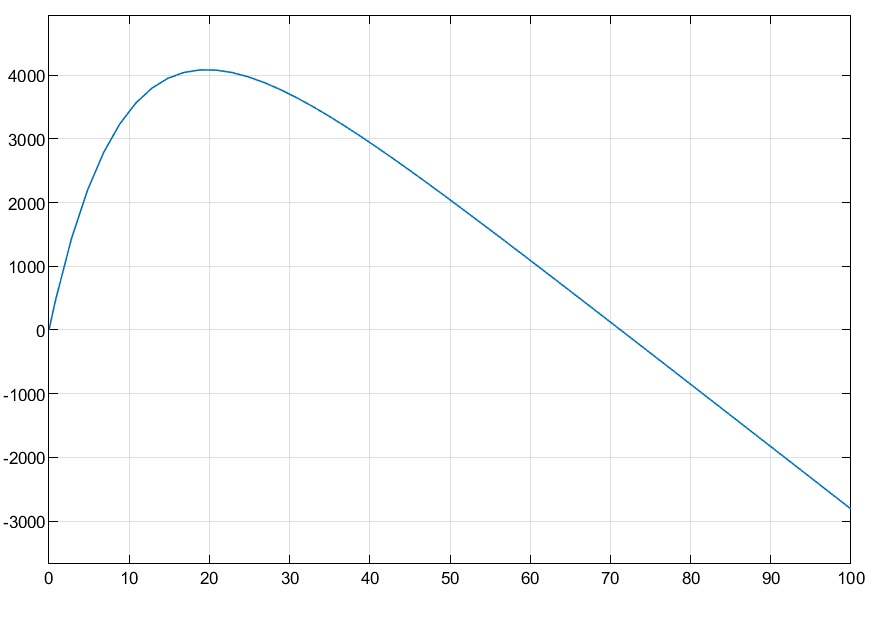
\includegraphics[width=0.7\linewidth]{graphy}
		\caption{Высота снаряда в зависимости от времени}
		\label{fig:graphvy}
	\end{figure}
	\begin{figure}[H]
		\centering
		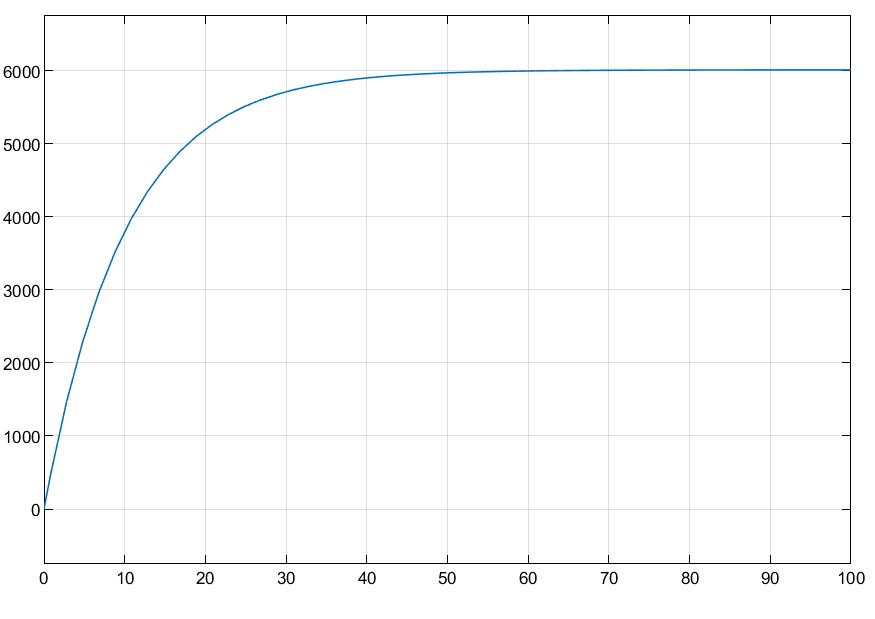
\includegraphics[width=0.7\linewidth]{graphx}
		\caption{Дальность полета в зависимости от времени}
		\label{fig:graphx}
	\end{figure}
	\begin{figure}[H]
		\centering
		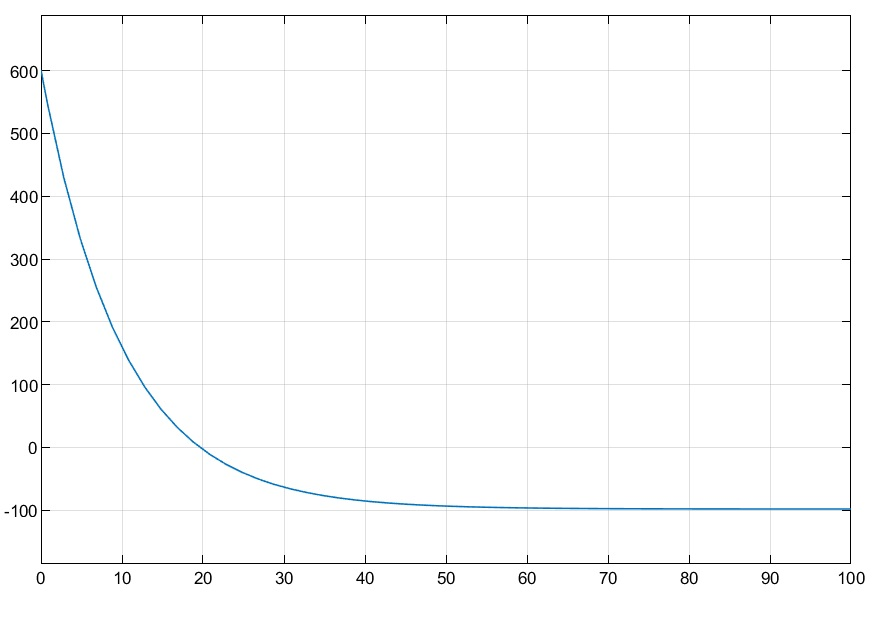
\includegraphics[width=0.7\linewidth]{graphvy}
		\caption{Скорость снаряда по вертикали в зависимости от времени}
		\label{fig:graphvy}
	\end{figure}
	\section{Выводы}
	\begin{enumerate}
		\item Максимальная дальность была достигнута при угле 45 градусов. При меньших углах траектория становится более пологой, падает высота и дальность.\\
		При больших углах растет максимальная высота, траектория становится более крутой, дальность падает.\\
		\begin{figure}[H]
			\centering
			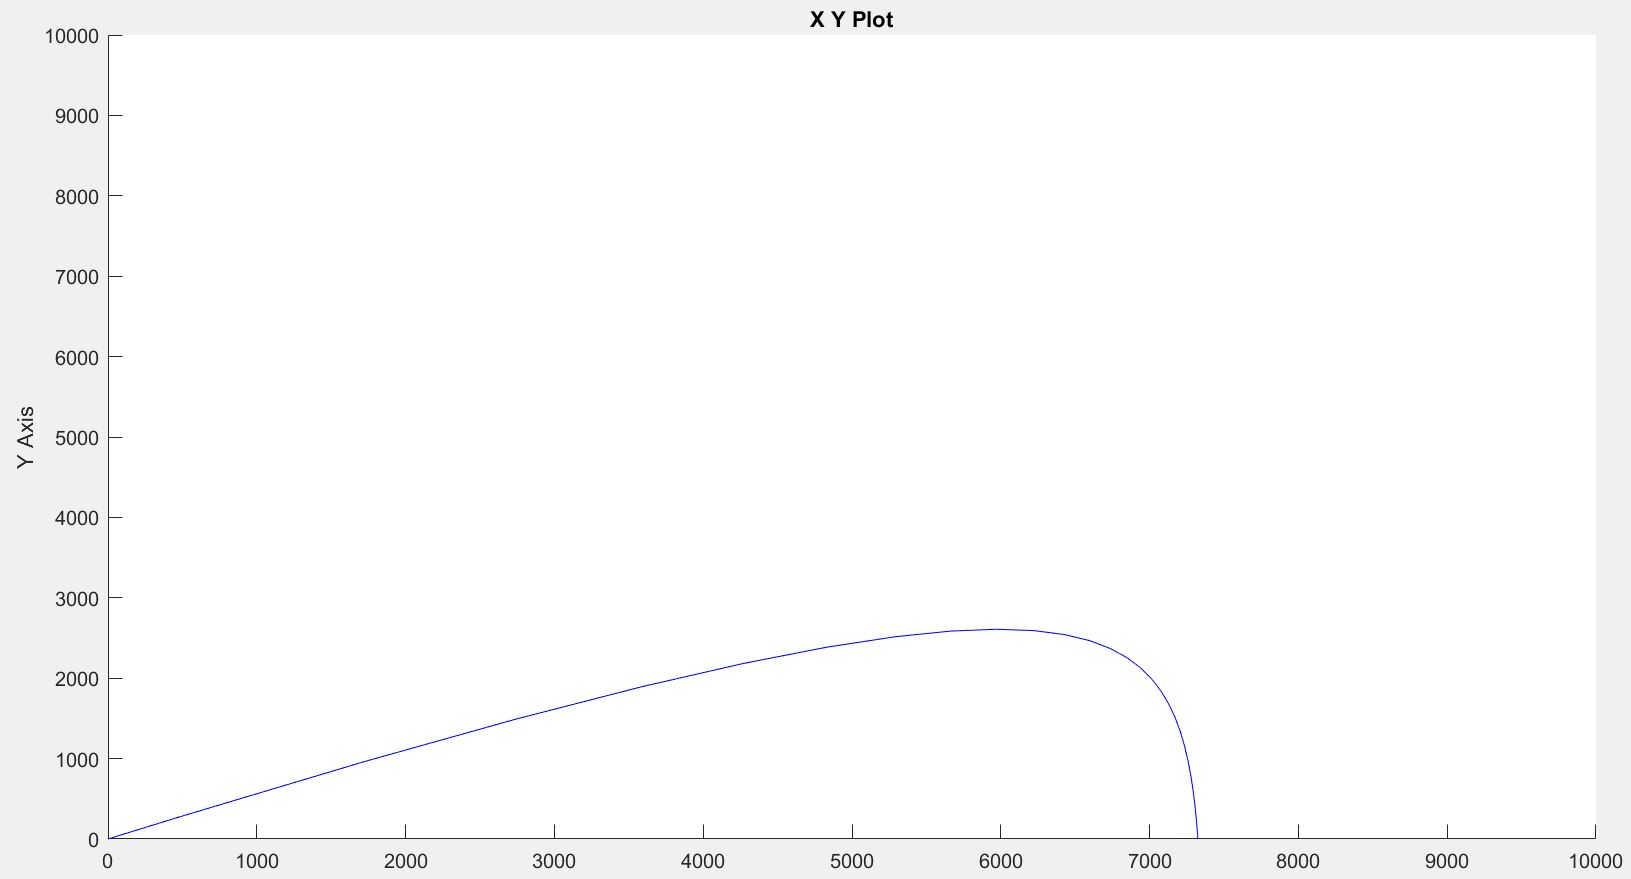
\includegraphics[width=0.7\linewidth]{graph2}
			\caption{Пологая траектория}
			\label{fig:graph2}
		\end{figure}
		\begin{figure}[H]
			\centering
			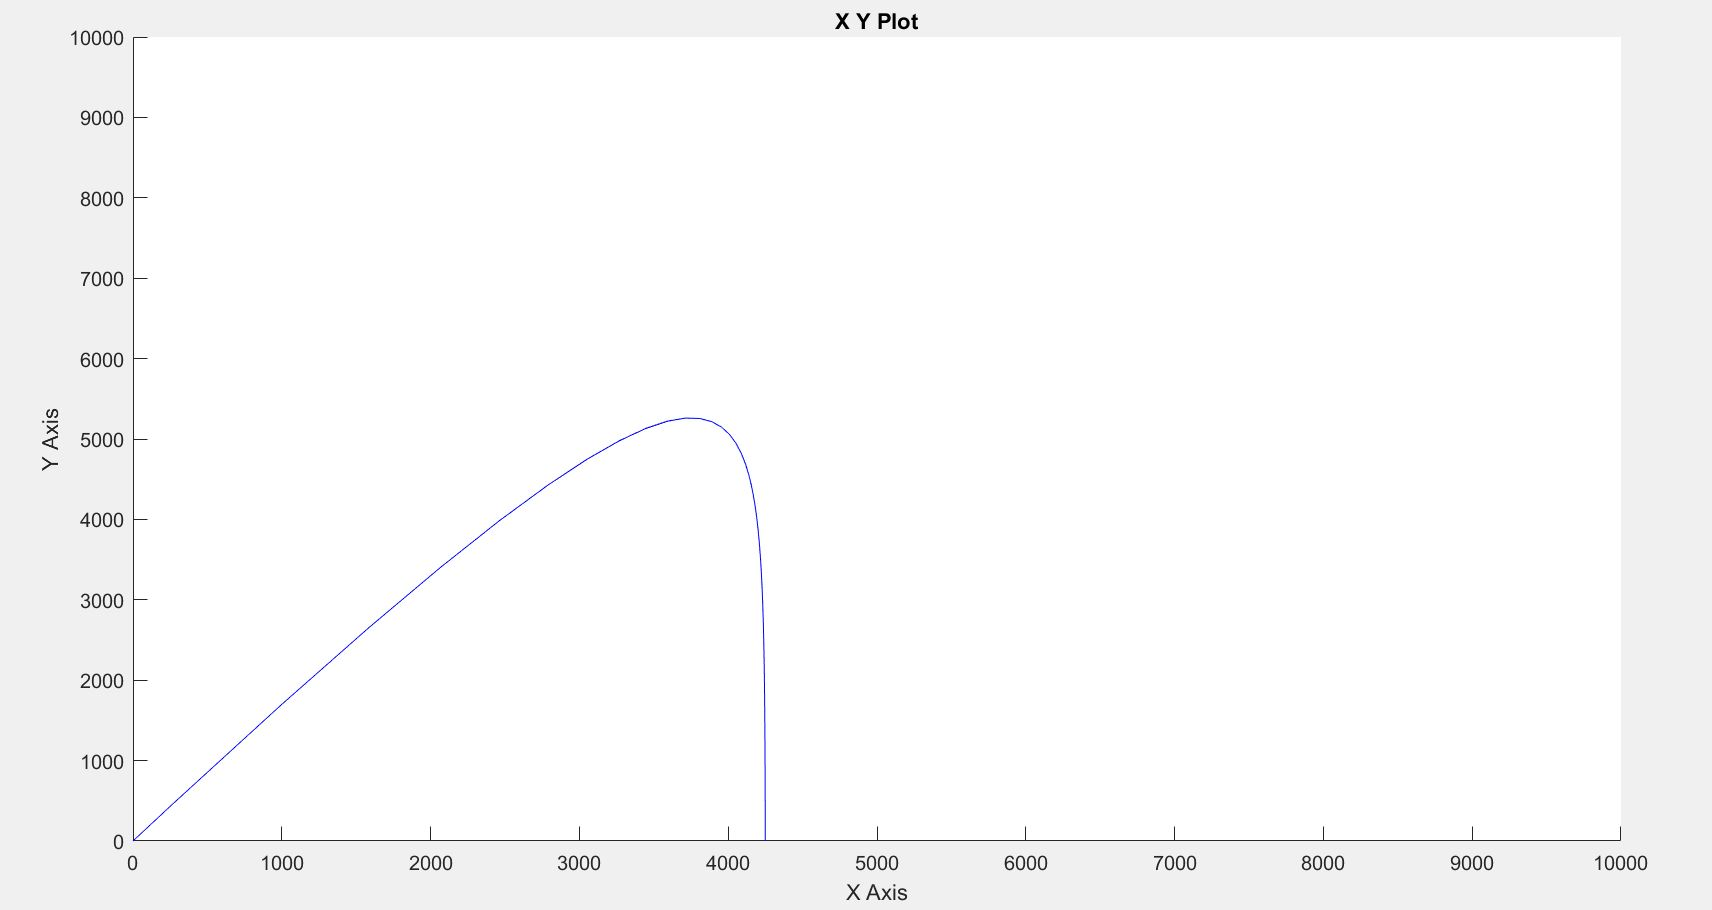
\includegraphics[width=0.7\linewidth]{graph3}
			\caption{Крутая траектория}
			\label{fig:graph3}
		\end{figure}
	\item Наибольшее влияние на дальность полета оказывают скорость и масса. Этот вывод не только подтверждается результатами моделирования, но и следует из формулы кинетической энергии тела.
	\end{enumerate}
	
\end{document}